\question{
  \item Considere a rede da figura sobre a qual opera um protocolo vetor-distância.

  \begin{figure}[H]
    \centering
    \includesvg[width=0.3\textwidth]{assets/011.svg}
  \end{figure}
}

\begin{enumerate}[leftmargin=\labelsep]
  \subquestion{
  \item No instante $t_0$ o protocolo está estável, com todos os nós a saber os
        comprimentos dos caminhos mais curtos para alcançar cada um dos outros nós. Apresente
        as entradas das tabelas de encaminhamento no que diz respeito ao nó destino $D$.
        }

        No instante inicial:

        \begin{itemize}
          \item $A$ sabe que o caminho mais curto para $D$ é direto, com custo 1.
          \item $B$ sabe que o caminho mais curto para $D$ tem próximo passo $A$, com custo total 3.
          \item $C$ sabe que o caminho mais curto para $D$ tem próximo passo $A$, com custo total 2.
          \item $D$ para $D$ é direto, com custo 0.
        \end{itemize}

        \subquestion{
  \item No instante $t_1$ a ligação $A-D$ falha. Assumindo que os nós trocam mensagens
        sincronamente em instantes bem definidos, $t_1, t_2, t_3, ...$, mostre a evolução das
        tabelas de encaminhamento até que o protocolo volte a estabilizar.
        }

        Inicialmente, todas as tabelas de custo tinham o seguinte aspeto (para todos os nós):

        \begin{table}[H]
          \centering
          \begin{tabular}{l|l|l|l|l}
            From/Cost to & A, $\pi$ & B, $\pi$ & C, $\pi$ & D, $\pi$ \\ \hline
            A            & 0        & 2, B     & 1, C     & 1, D     \\
            B            & 2, A     & 0        & 2, C     & 3, A     \\
            C            & 1, A     & 2, B     & 0        & 2, A     \\
            D            & 1, A     & 3, A     & 2, A     & 0
          \end{tabular}
        \end{table}

        Após a ligação $A-D$ falhar, as tabelas vão sendo progressivamente atualizadas,
        como se segue:

        \begin{figure}[H]
          \centering
          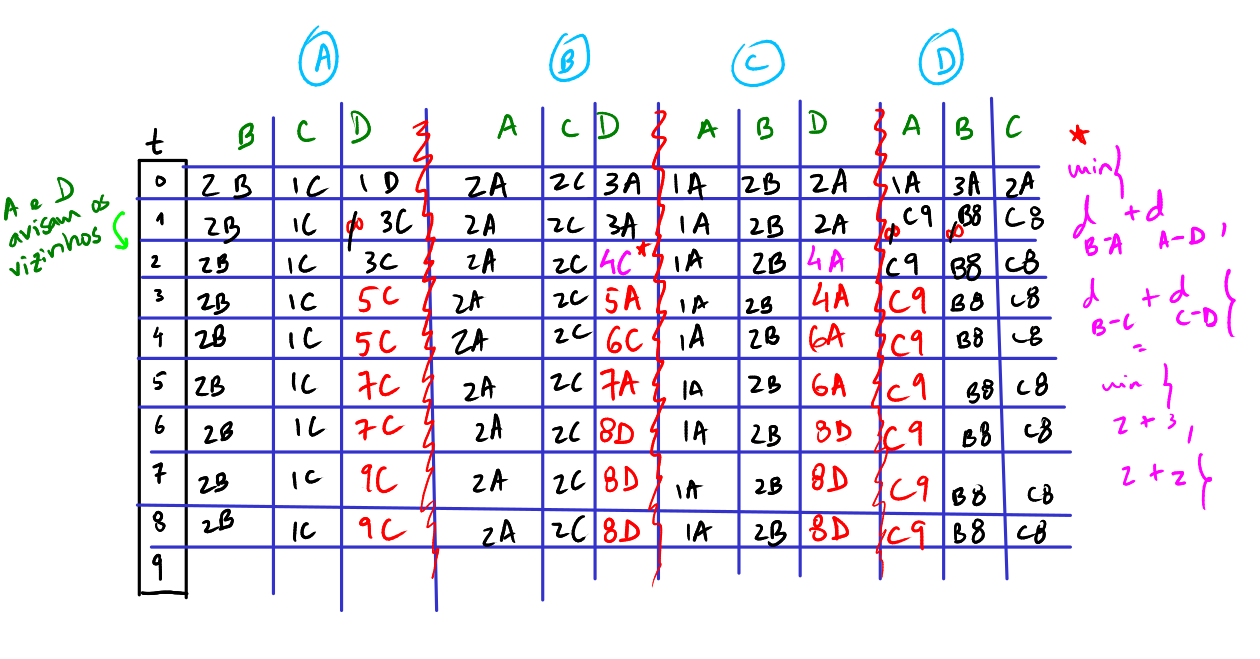
\includegraphics[width=0.7\textwidth]{assets/011b.png}
        \end{figure}

        \subquestion{
  \item Repita a alínea anterior, mas assumindo agora que o protocolo utilizado é
        vetor-caminho. Neste protocolo os nós trocam entre si não apenas a distância para
        alcançar cada destino mas também todo o caminho (sequência de nós) associado a essa distância.
        }

        \dots (acabo depois)
\end{enumerate}